\documentclass[tikz,border=0.5mm,svgnames]{standalone}
\usepackage{tkz-euclide}
\usetikzlibrary{backgrounds}
\def\nodecolor{LightSteelBlue}
\def\nodesize{0.3}

\tikzset{arrow/.style={
  decoration={markings,
  mark=at position .5 with {\arrow[scale=2]{>}}},
  >=stealth,
}}

\tkzSetUpLine[line width=1.5pt] 

\tikzset{pics/state/.style args={#1/#2/#3/#4/#5}{code={
    \tkzDefPoint(0,0){A}
    \tkzDefPoint(2,0){B}
    \tkzDefTriangle[equilateral](A,B)\tkzGetPoint{C}
    \tkzDrawPolygon(A,B,C)
    \tkzDefPoint(4,0){D}
    \tkzDefTriangle[equilateral](B,D)\tkzGetPoint{E}
    \tkzDrawSegments[Red](B,A C,B A,C B,E D,B E,D)
    \tkzDefCircle[R](A,\nodesize)\tkzGetPoint{XA} \tkzDrawCircle[fill=\nodecolor](A,XA)
    \tkzDefCircle[R](B,\nodesize)\tkzGetPoint{XB} \tkzDrawCircle[fill=\nodecolor](B,XB)
    \tkzDefCircle[R](C,\nodesize)\tkzGetPoint{XC} \tkzDrawCircle[fill=\nodecolor](C,XC)
    \tkzDefCircle[R](D,\nodesize)\tkzGetPoint{XD} \tkzDrawCircle[fill=\nodecolor](D,XD)
    \tkzDefCircle[R](E,\nodesize)\tkzGetPoint{XE} \tkzDrawCircle[fill=\nodecolor](E,XE)
    \tkzLabelPoint[anchor=center](A){#1}
    \tkzLabelPoint[anchor=center](B){#2}
    \tkzLabelPoint[anchor=center](C){#3}
    \tkzLabelPoint[anchor=center](D){#4}
    \tkzLabelPoint[anchor=center](E){#5}
}}}%  

\tikzset{pics/X/.style args={#1}{code={
    \begin{scope}[on background layer]
    \tkzDrawSegments[Red,arrow,postaction={decorate}](B,A C,B A,C)
    \end{scope}
}}}%  

\tikzset{pics/Y/.style args={#1}{code={
    \begin{scope}[on background layer]
    \tkzDrawSegments[Red,arrow,postaction={decorate}](B,E D,B E,D)
    \end{scope}
}}}%  

\begin{document}

% 1. Notation: absolute node positions
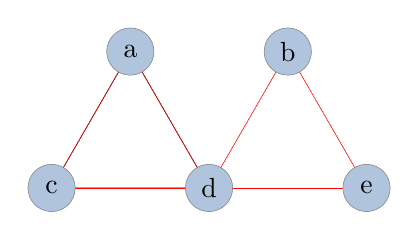
\begin{tikzpicture}
  \pic {state=c/d/a/e/b};
  %\pic {X};
  %\pic {Y};
\end{tikzpicture}

% 2. Initial state
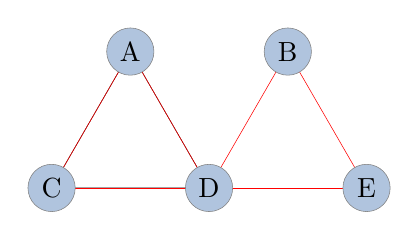
\begin{tikzpicture}
  \pic {state=C/D/A/E/B};
\end{tikzpicture}

% 3. Part (a) - Final state
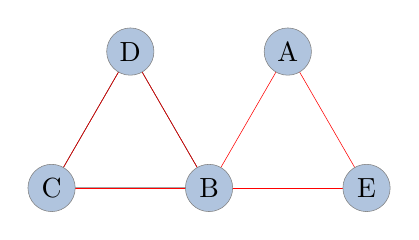
\begin{tikzpicture}
  \pic {state=C/B/D/E/A};
\end{tikzpicture}


% 4. Part (b) - Intermediate state
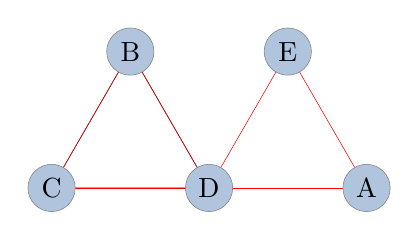
\begin{tikzpicture}
  \pic {state=C/D/B/A/E};
\end{tikzpicture}

% 5. A move
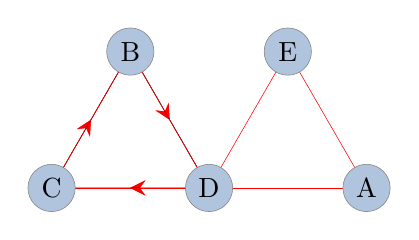
\begin{tikzpicture}
  \pic {state=C/D/B/A/E};
  \pic {X};
\end{tikzpicture}

\end{document}
